
\section{Introduction}
\label{sec:introduction}

The study of the evolution of galaxies and the growth of the supermassive black holes at their cores go hand in hand.  Although the typical length scales for the two can vary by many orders of magnitude, they seem inexorably linked.  Observational correlations between galaxy and supermassive black hole properties hint at an underlying co-evolution driven by shared mechanisms.



%%%%%%%%%%%%%%%%%%%%%%%%%%%%%%%%%%%%%%%%%%%%%%%%%%%%
\subsection{Galaxy Properties}

How do we describe a galaxy?  Being extended, resolvable objects, galaxies provide a unique wealth of observable characteristics not obtainable from point sources such as stars.  While many characteristics can be deduced about point sources, the actual observations themselves come down to measuring position on the sky and measuring flux as a function of frequency and time.  From this information, all that we know about stars and other point sources, such as temperature, age, size, and composition, can be inferred.  However, for extended objects like galaxies, we are given more to work with.


%---------------------------------------------------
\subsubsection{Color}

A galaxy's color is determined by its stellar component.  While a galaxy in itself may be resolvable, for all but the most nearby of galaxies, individual stars are not.  What we see when looking at a particular small section of a galaxy is the averaged-together light from stars in that section.

Broadly, bluer late-type spirals have a $u-r$ color of around $1.3 - 2.0$, while redder early-type galaxies have a $u - r$ color of around $2.3 - 2.7$.  The color of a galaxy can be a good indicator for its age and evolutionary stage.  Star formation processes generally tend to produce many smaller, cooler, redder stars and fewer larger, hotter, bluer stars.  These small, cool stars are much longer-lived than their massive counterparts, while the large, warm stars are much brighter.  After star formation turns off, the short-lived blue stars begin to die off, and the galaxy becomes redder, as more of the fraction of total light comes from the red end of the population.



%---------------------------------------------------
\subsubsection{Morphology}

The extended nature of galaxies allows us to observe their morphology.  The classification scheme originally devised by \citet{hubble_1926} places galaxies into the four broad categories:  elliptical, spiral, lenticular, and irregular.  Elliptical galaxies tend to be larger, redder, have less gas, and dominated by more radial orbits.  Spiral galaxies tend to be smaller, bluer, have more gas, and have more of a disk component.  Spirals can have a number or arms, a central bulge, and a central bar.  Lenticular galaxies are middle-of-the-road galaxies, with both a strong central bulge like an elliptical, and an extended disk like a spiral, however without spiral arms.  Irregular galaxies tend to defy this simple classification scheme, and can be found in any number of configurations.

Figure~\ref{fig:tuning_fork} is a cartoon of the classification scheme.  To the left of the diagram are elliptical galaxies.  The subcategories are an indication of the shape of the galaxy, with the most spherical on the left and progressing to more flattened shapes to the right.  On the right of the diagram are spiral galaxies.  These are broken into two branches, based on whether or not the galaxy contains a central bar.  Moving from right to left, the spiral arms of the galaxies become more tightly wound, and the central bulges become more dominant.  At the center of the diagram where the spiral fork meets the elliptical line, lie lenticular galaxies.  Irregular galaxies are, as the name would imply, irregular and do not fall on the diagram.

\begin{figure}[t]
\centering
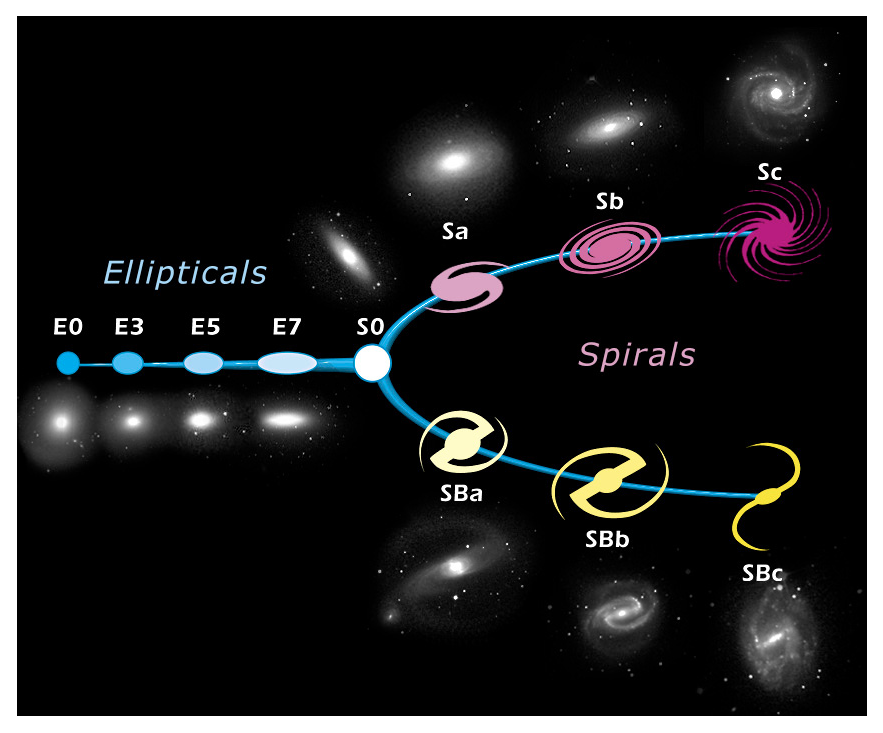
\includegraphics[width=0.75\linewidth]{hubble_tuning_fork.eps}
\caption[The Hubble tuning fork]{\footnotesize The Hubble tuning fork.  On the left of the diagram are elliptical galaxies.  E0 galaxies are the most spherical, while E7 are the most flattened or elongated.  S0 are lenticular galaxies.  The top branch on the right are spiral galaxies with no bar, while the bottom right branch are spiral galaxies with a bar.  Both progress from tightly wound spiral arms and large bulges to loosely wound spiral arms and small to no bulges, going from Sa to Sc or SBa to SBc.}
\label{fig:tuning_fork}
\end{figure}



%%%%%%%%%%%%%%%%%%%%%%%%%%%%%%%%%%%%%%%%%%%%%%%%%%%%
\subsection{Supermassive Black Hole Properties}

A non-merging black hole, much like an elementary particle, can be described simply by its mass, charge, and spin.  Its effect on its local spacetime, infalling matter, and surrounding environment all come back to these three parameters.  However, determination of these parameters and the study of how black holes interact with their surroundings can be quite involved.


%---------------------------------------------------
%\subsubsection{Observations}

Black holes are, by their very nature, black, and difficult to observe.  We cannot see light emitted directly from a black hole as we would a star, since a black hole is defined as an object massive and compact enough to not allow light within its event horizon to escape.  We are forced, therefore, to employ other methods of measuring black holes.

Thus far, the majority of progress in the measurement of black hole properties has been in measuring mass.  There are a number of ways to measure the mass of a black hole.  Here, we will briefly discuss masers, stellar dynamics, gas dynamics, and reverberation mapping as methods of measuring a supermassive black hole's mass.

Astrophysical masers are sources of stimulated spectral line emission in the microwave band formed in regions of high-density gas comprised of molecules such as hydroxyl, formaldehyde, and water \citep{lo_2005}.  Since the emission frequencies of these sources are very well constrained, high-accuracy Doppler shifts can be determined.  These Doppler shifts can then be used to determine velocities for the masers, and thus how much mass is enclosed by their orbits.  If these masers lie very close to the supermassive black hole (SMBH) in the center of their galaxy, the enclosed mass can be constrained to be primarily that of the SMBH.

\begin{figure}[t]
\centering
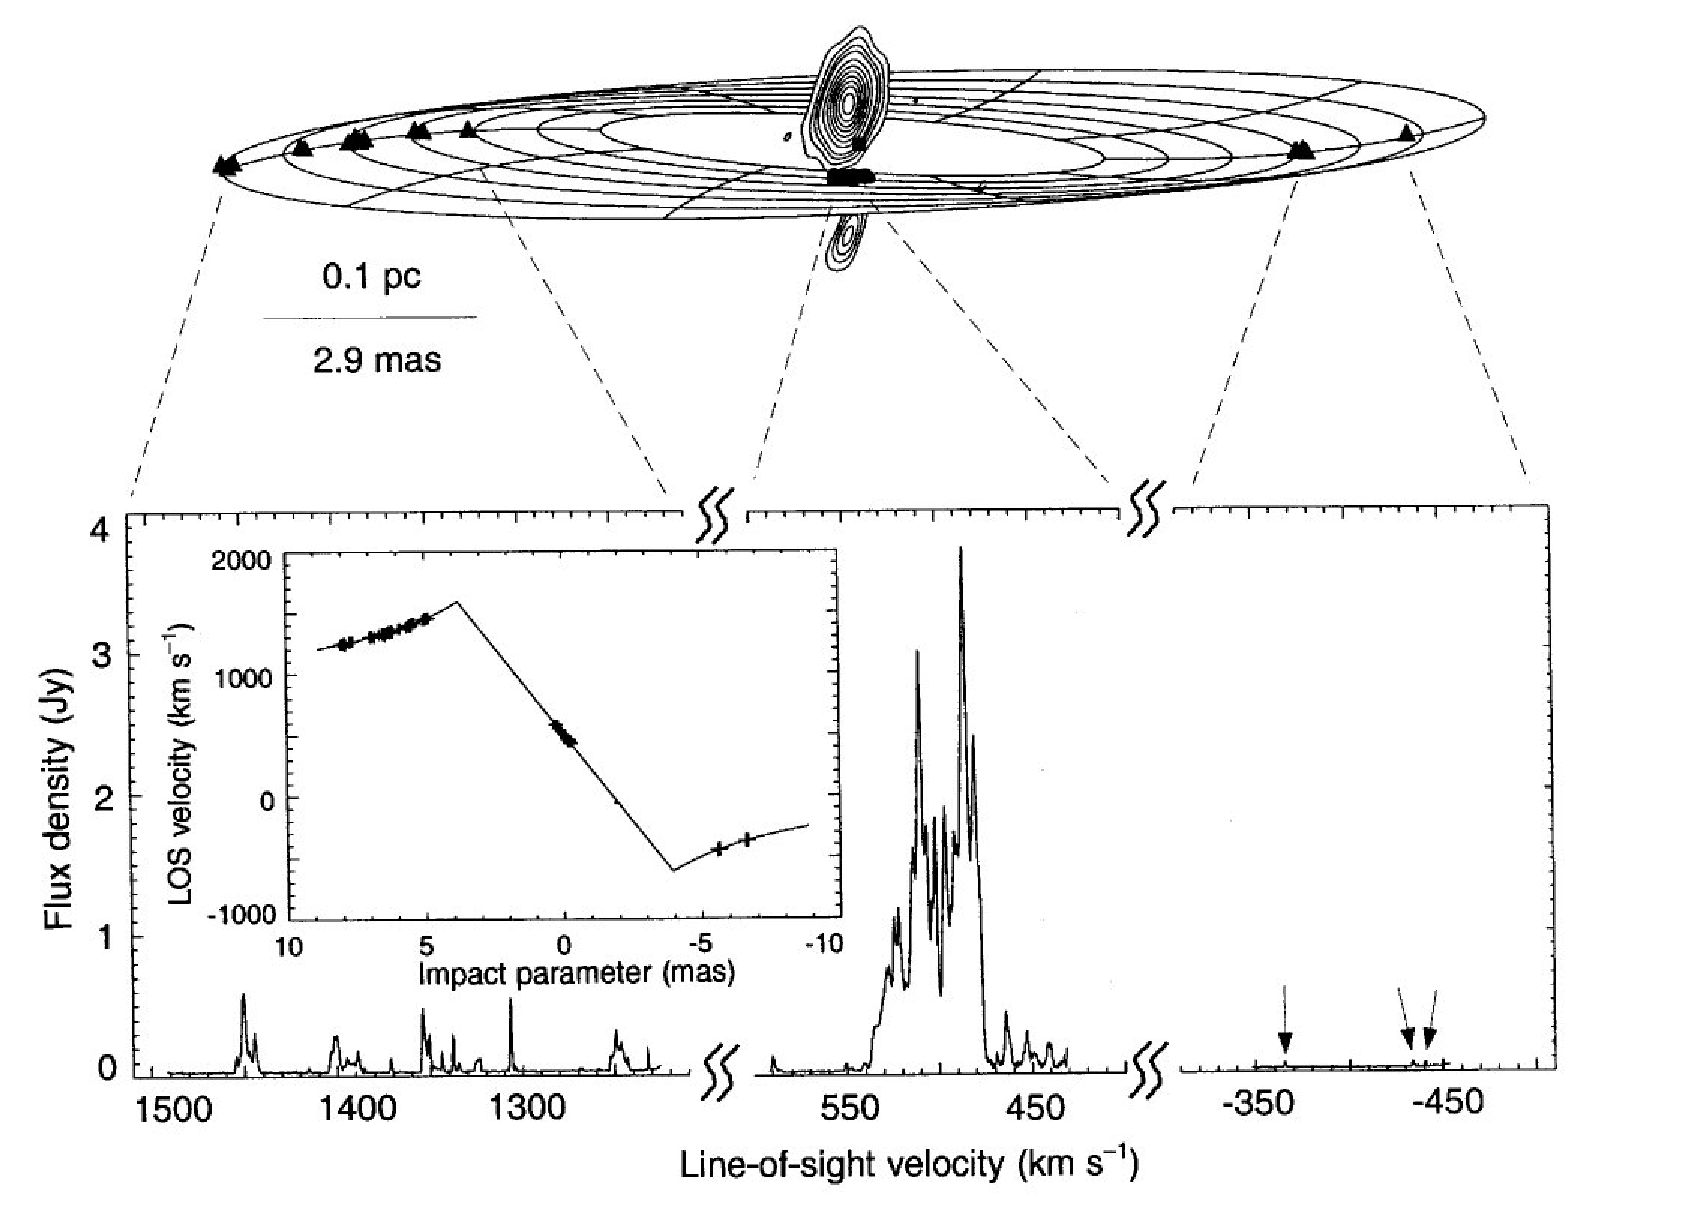
\includegraphics[width=\linewidth]{herrnstein_1999_masers.eps}
\caption[Maser orbits fit to a warped disk for NGC4258]{\footnotesize Maser orbits fit to a warped disk for NGC4258.  Masers can also be useful for distance determinations.  Here, the positions and velocities of water masers are able to be fit to a warped disk model surrounding a supermassive black hole.  This allows the interpolation of physical radii away from the black hole, giving us both the black hole mass and an standard ruler to allow precise determination of the distance to NGC4258.  \citep{herrnstein_1999}}
\label{fig:masers}
\end{figure}

Stellar dynamics and gas dynamics both probe light coming from matter near the black hole.  The width of broadened spectral lines from either the stars or gas can be used to determine a velocity dispersion for the matter local to the SMBH.  This velocity dispersion, therefore, can then be used to determine the potential through which the matter is traveling, and thus the mass of the black hole.

A special case of stellar dynamics for which the orbits of the constituent stars can be resolved---namely, for the case of our own Milky Way---adds another dimension to our knowledge of the stellar orbits.  Over time, we can observe the proper motion on the sky for these orbits.  Combining these measurements with Doppler measurements for radial velocity yields full orbital solutions.  Then, it simply requires Kepler's laws to determine the mass of the SMBH.

Reverberation mapping can be thought of as ``echo-mapping'' the gas disk around a SMBH.  Continuum emission very near the black hole travels outward and stimulates broad line emission in surrounding gas.  Any changes in the continuum emission will take time to propagate to the broad line region, since the speed of light is finite.  By measuring the timing difference in the change in continuum emission and change in stimulated broad line emission, the physical distance from the SMBH to the broad line region can be inferred.  With this radius, and the velocity of the gas in the broad line region measured by the width of the broadened lines, a black hole mass can be determined \citep{blandford_1982}.



%%%%%%%%%%%%%%%%%%%%%%%%%%%%%%%%%%%%%%%%%%%%%%%%%%%%
\subsection{Correlations}

Correlations between varying properties of galaxies and black holes can provide much deeper insight into the dynamics that shape the evolution of both.  Of particular interest here are the fundamental plane of elliptical galaxies, the $M-\sigma$ relation, and the green valley-AGN relation.


%---------------------------------------------------
\subsubsection{The M-Sigma Relation}

If we consider the all the observable properties of a galaxy and compare them to the mass of its SMBH, the tightest correlation can be found with the velocity dispersion $\sigma$ of the galaxy's bulge.  Such a tight correlation is surprising, as the sphere of influence of a typical SMBH does not extend much past order a few pc, while bulges exist on scales of a kpc or greater.  In essence, the supermassive black hole and the outer edges of the bulge shouldn't ``feel'' each other.  Nevertheless, the correlation is indeed there, suggesting some mechanism that influences---or is influenced by---both of them.  \citet{gultekin_2009a} use a sample of 49 $M_{BH}$ measurements and 19 upper limits to measure this correlation, and find $\log(M_{BH}/M_{\odot}) = \alpha + \beta \log(\sigma/200$~km~s$^{-1})$ with $(\alpha, \beta, \epsilon_{0}) = (8.12 \pm 0.08 M_{\odot}, 4.24 \pm 0.41 M_{\odot}, 0.44 \pm 0.06 M_{\odot})$ for all galaxies and $(\alpha, \beta, \epsilon_{0}) = (8.23 \pm 0.08 M_{\odot}, 3.96 \pm 0.42 M_{\odot}, 0.31 \pm 0.06 M_{\odot})$ for ellipticals, where $\epsilon_{0}$ is the intrinsic scatter in the relation.

\begin{figure}[tp]
\centering
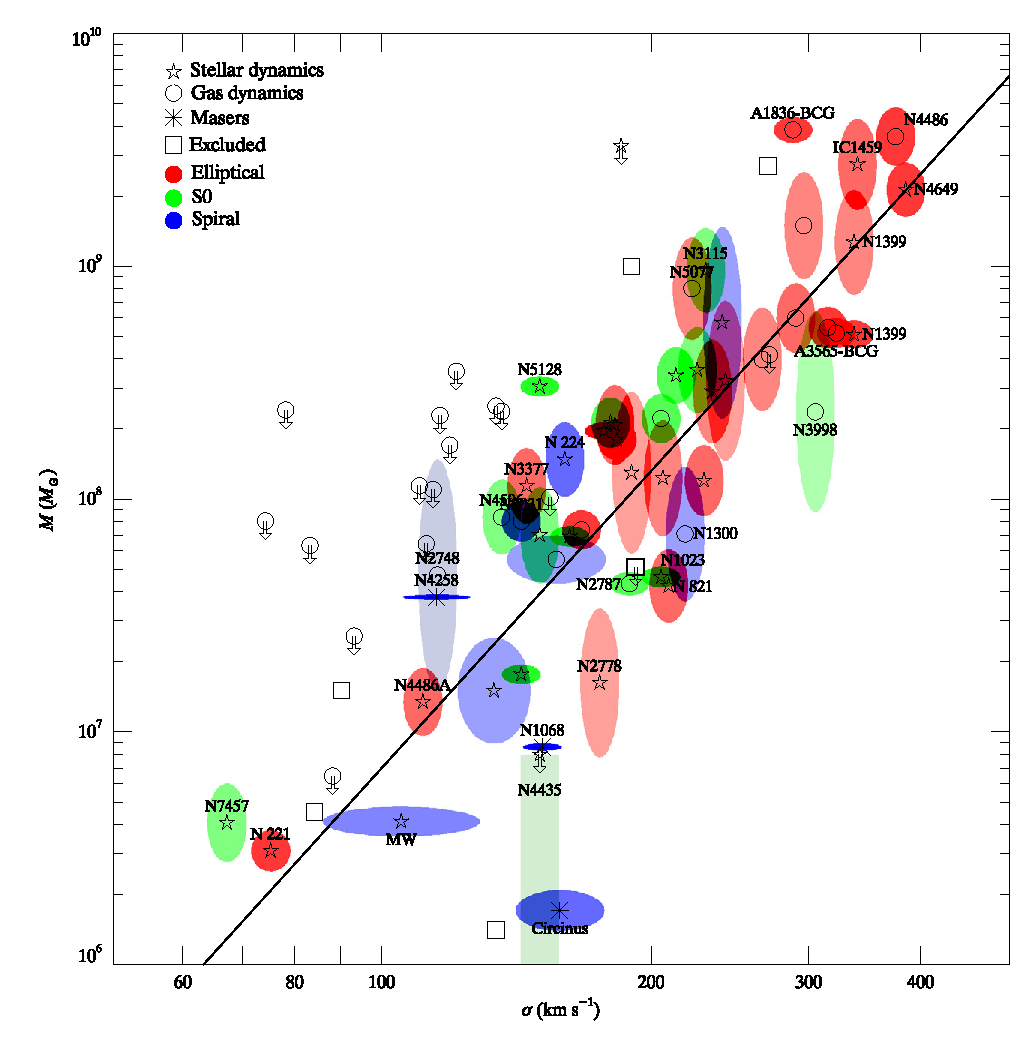
\includegraphics[width=\linewidth]{gultekin_2009a_m-sigma.eps}
\caption[The M-$\sigma$ relation for galaxies with dynamical measurements]{\footnotesize The M-$\sigma$ relation for galaxies with dynamical measurements.  Black hole mass is plotted vs velocity dispersion of its host spheroid.  The symbols represent the method by which the black hole mass was measured:  pentagrams for stellar dynamics, circles for gas dynamics, and asterisks for masers.  Upper limits are given by arrows.  Error ellipses are colored by galaxy type, with red for ellipticals galaxies, green for lenticular galaxies, and blue for spiral galaxies.  The saturation of the color is inversely proportional to the area of the ellipse.  For this sample, the best fit relation is $M_{BH} = 10^{8.12}$ M$_{\odot} (\sigma / 200$ km s$^{-1})^{4.24}$.  Galaxies not included in this fit are labeled as squares.  \citep{gultekin_2009a}}
\label{fig:m-sigma}
\end{figure}


%---------------------------------------------------
\subsubsection{The Fundamental Plane}

While not a direct correlation with the properties of supermassive black holes, the fundamental plane of elliptical galaxies offers insight into the characteristics of their hosts.  The fundamental plane is a three-parameter correlation between properties of elliptical galaxies:  velocity dispersion, effective radius, and surface brightness.  This correlation (Figure \ref{fig:fundamental_plane}) between these three parameters is tighter than the combination of any two alone \citep{djorgovski_1987}.  The fit for this correlation can be given as $\log R_{e} = 0.36(\langle I \rangle_{e} / \mu_{B}) + 1.4 \log \sigma_{0}$, where $R_{e}$ is the effective radius in kpc, $\langle I \rangle_{e}$ is the mean surface brightness interior to $R_{e}$ in units of $\mu_{B}$, and $\sigma_{0}$ is the velocity dispersion in km s$^{-1}$ \citep{binney_merrifield_1998}.

\begin{figure}[tp]
\centering
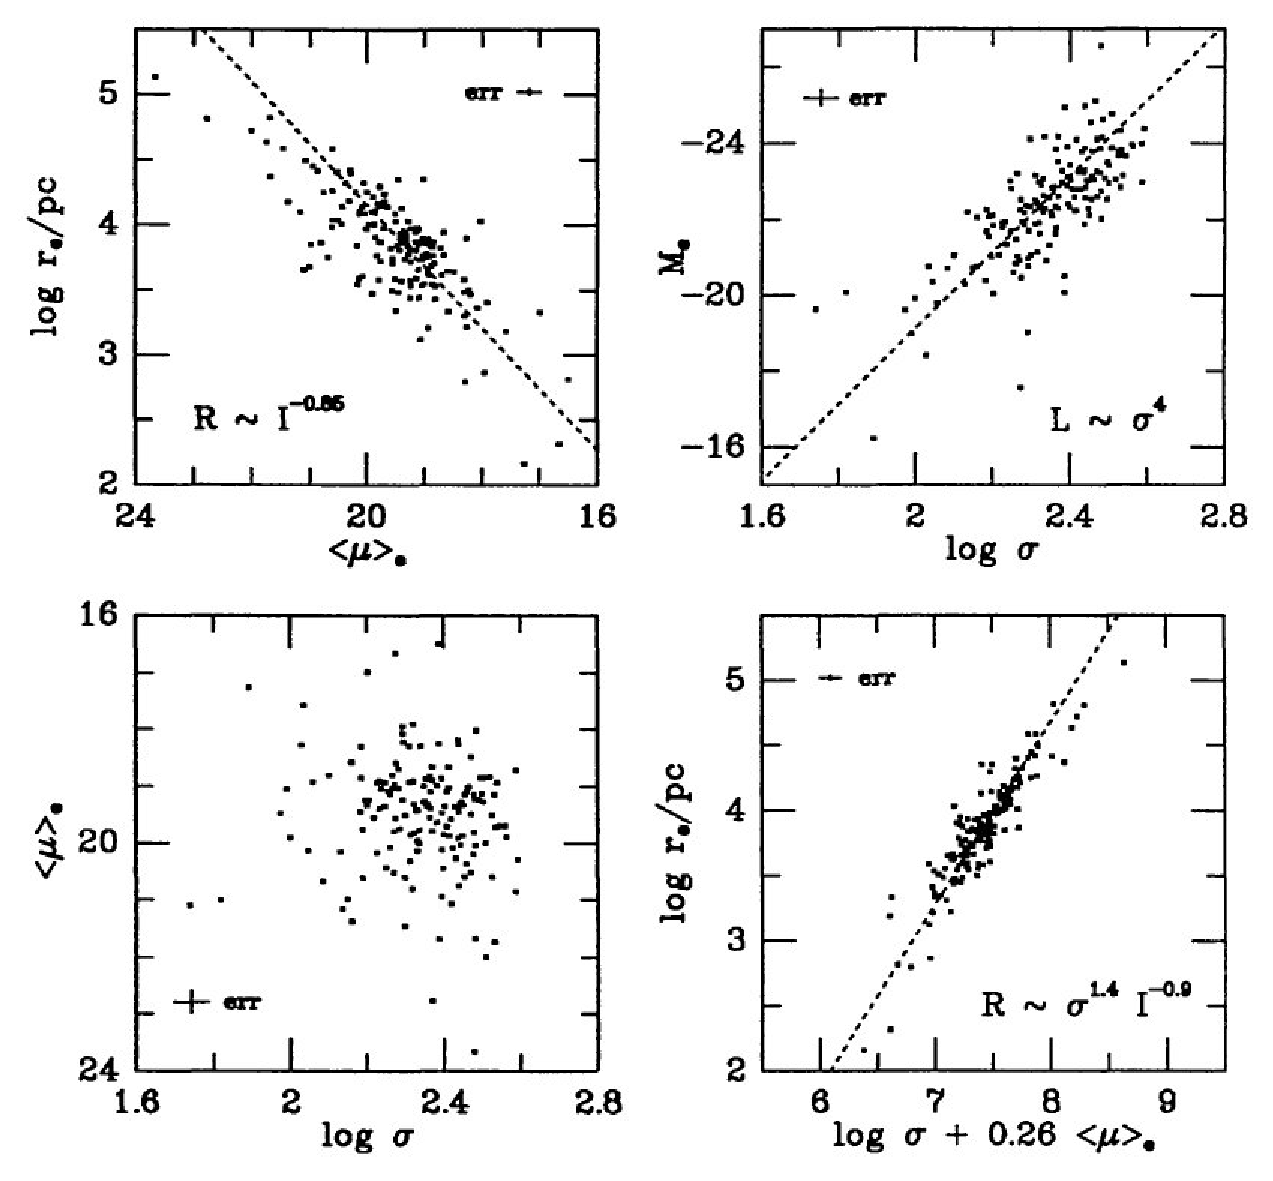
\includegraphics[width=\linewidth]{kormendy_1989_fundamental_plane.eps}
\caption[The fundamental plane for elliptical galaxies]{\footnotesize The fundamental plane for elliptical galaxies.  \textit{Top panels:} The top panels show the one-parameter scaling relations, with the relation between radius and mean surface brightness on the left and the relation between luminosity and velocity dispersion (the Faber-Jackson relation) on the right.  \textit{Bottom left:} The relation between the surface brightness and velocity dispersion.  This is an almost face-on view of the fundamental plane.  \textit{Bottom right:} The relation between the effective radius and the combination of surface brightness and velocity dispersion.  This is the edge-on view of the fundamental plane.  \citep{kormendy_1989}}
\label{fig:fundamental_plane}
\end{figure}


%---------------------------------------------------
\subsubsection{The Green Valley}

When considering both the color and stellar mass of a galaxies, a correlation emerges where many galaxies lie in either the ``blue cloud'' of bluer, lower mass galaxies, or the ``red sequence'' of redder, generally higher mass galaxies.  The area between these two is known as the ``green valley'' and, while not as populated as the blue cloud or red sequence, holds special interest when active galactic nuclei (AGN) are considered.  AGN are very luminous regions at the centers of some galaxies.  \citet{schawinski_2010} show that galaxies falling on the green valley are much more likely to host AGN than galaxies on the blue cloud or red sequence, hinting at an underlying link between the evolution of galaxies, and the activity at their centers.

\begin{figure}[t]
\centering
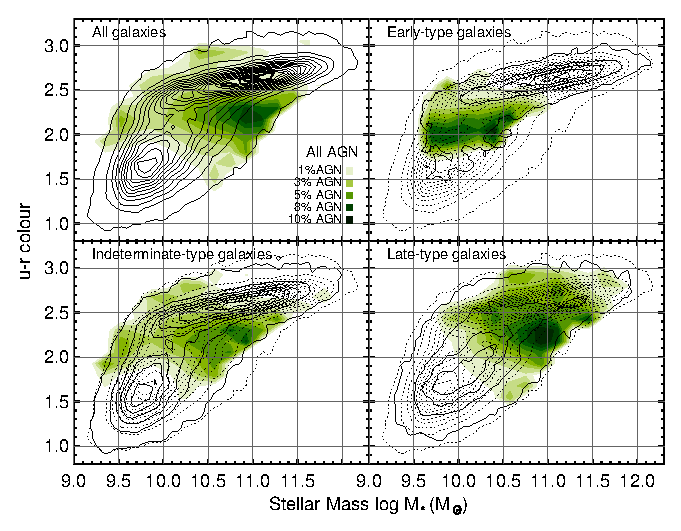
\includegraphics[width=\linewidth]{schawinski_2010_green_valley.eps}
\caption[Distribution of the fraction of galaxies containing AGN]{\footnotesize Distribution of the fraction of galaxies containing AGN.  Galaxy color in u-r is plotted vs stellar mass.  The contours are the galaxy population for all galaxies (top-left), early-type galaxies (top right), intermediate-type galaxies (bottom left), and late type galaxies (bottom right).  For the three sub-samples, dotted contours represent the full sample for comparison.  The green shaded contours represent the fraction of galaxies in that subsample that contain active galactic nuclei.  It can be clearly seen that the AGN fraction is highest for galaxies falling within the green valley.  \citep{schawinski_2010}}
\label{fig:green_valley}
\end{figure}



